%=======================================================
%	PACKAGES AND THEMES
%=======================================================
\documentclass[8pt]{beamer}
\mode<presentation> {
\usepackage{etex}
\usetheme{Boadilla}
\definecolor{navyblue}{rgb}{0.0, 0.0, 0.5}
\definecolor{dkgreen}{rgb}{0,0.6,0}
\definecolor{gray}{RGB}{64, 64, 64}
\definecolor{teal}{RGB}{0, 102, 102}
\definecolor{mauve}{rgb}{0.58,0,0.82}
\usecolortheme[named = navyblue]{structure}
\setbeamercolor{normal text}{fg = gray}
\setbeamercolor{frametitle}{fg = white, bg = navyblue}
\setbeamerfont{framesubtitle}{size = \normalsize}
\setbeamerfont{caption}{size=\footnotesize}
\setbeamercolor{page number in head/foot}{fg = gray}
\setbeamertemplate{footline}%[frame number]
}


\usepackage{graphicx} % Allows including images
\usepackage{booktabs} % Allows the use of \toprule, \midrule and \bottomrule in tables
\usepackage{multicol}
\usepackage[export]{adjustbox}
\usepackage{colortbl}
\usepackage{graphicx} 
\usepackage{etoolbox}

\usepackage{tikz}
\usepackage{fancybox}
\usepackage[absolute, overlay]{textpos}
\usepackage{multirow}
\usepackage{siunitx}
\usepackage{tcolorbox}


\usepackage{tikz}
\usepackage{calc}
\newlength{\outerradius}
\newlength{\innerradius}
\setlength{\outerradius}{0.50cm}
\setlength{\innerradius}{0.35cm}

%=======================================================
%	TITLE PAGE
%=======================================================


\title{\textbf{Introduction}}

\author{Dr David Eggleton}

\institute
{
SPRU (Science Policy Research Unit) \\
Business School\\
University of Sussex \\

\medskip

\medskip

\medskip

\includegraphics[width=2.5cm]{../_shared_pics/logo}

\medskip

\textit{{\color{dkgreen}{Week 1}}}\\
}


\date{} % Date, can be changed to a custom date

\begin{document}

\begin{frame}
\titlepage % Print the title page as the first slide

\begin{textblock*}{10pt}(0pt, 0.9\textheight)
\includegraphics[width=4cm]{../_shared_pics/SPRU.png}
\end{textblock*}

\end{frame}




%=======================================================
%	Intro slides
%=======================================================

\begin{frame}
\frametitle{Overview}
\tableofcontents[hideallsubsections]
\end{frame}

%------------------------------------------------

\begin{frame}
\frametitle{Teaching team}


\begin{columns}[c]
\column{.45\textwidth}
\centering
\includegraphics[width = \textwidth]{team2}\\
\tiny{Source: Linkedin}

\column{.45\textwidth}
\textbf{David Eggleton}\\
Convenorship, Lectures\\
(d.eggleton@sussex.ac.uk)

\bigskip

\textbf{Yongyuan Huang}\\
Seminars\\
(yongyuan.huang@sussex.ac.uk)

\end{columns}

\end{frame}

%------------------------------------------------

\begin{frame}
\frametitle{The future experts of Network Analysis and Infographics ...}

Please introduce yourself

\begin{itemize}
	\item Name and MSc course
	\item Why did you choose this module?
	\item What do you expect to achieve at the end of this module?
\end{itemize}

\end{frame}

%------------------------------------------------



	
%=======================================================
%	Why network analysis?
%=======================================================
\section{Why network analysis?}

%------------------------------------------------

\bgroup
\setbeamercolor{background canvas}{bg = navyblue}
\begin{frame}[plain]{}
\begin{center}
\color{white}{\Huge \insertsection}
\end{center}
\end{frame}
\egroup

%------------------------------------------------

\begin{frame}
\frametitle{\insertsection}
\centering
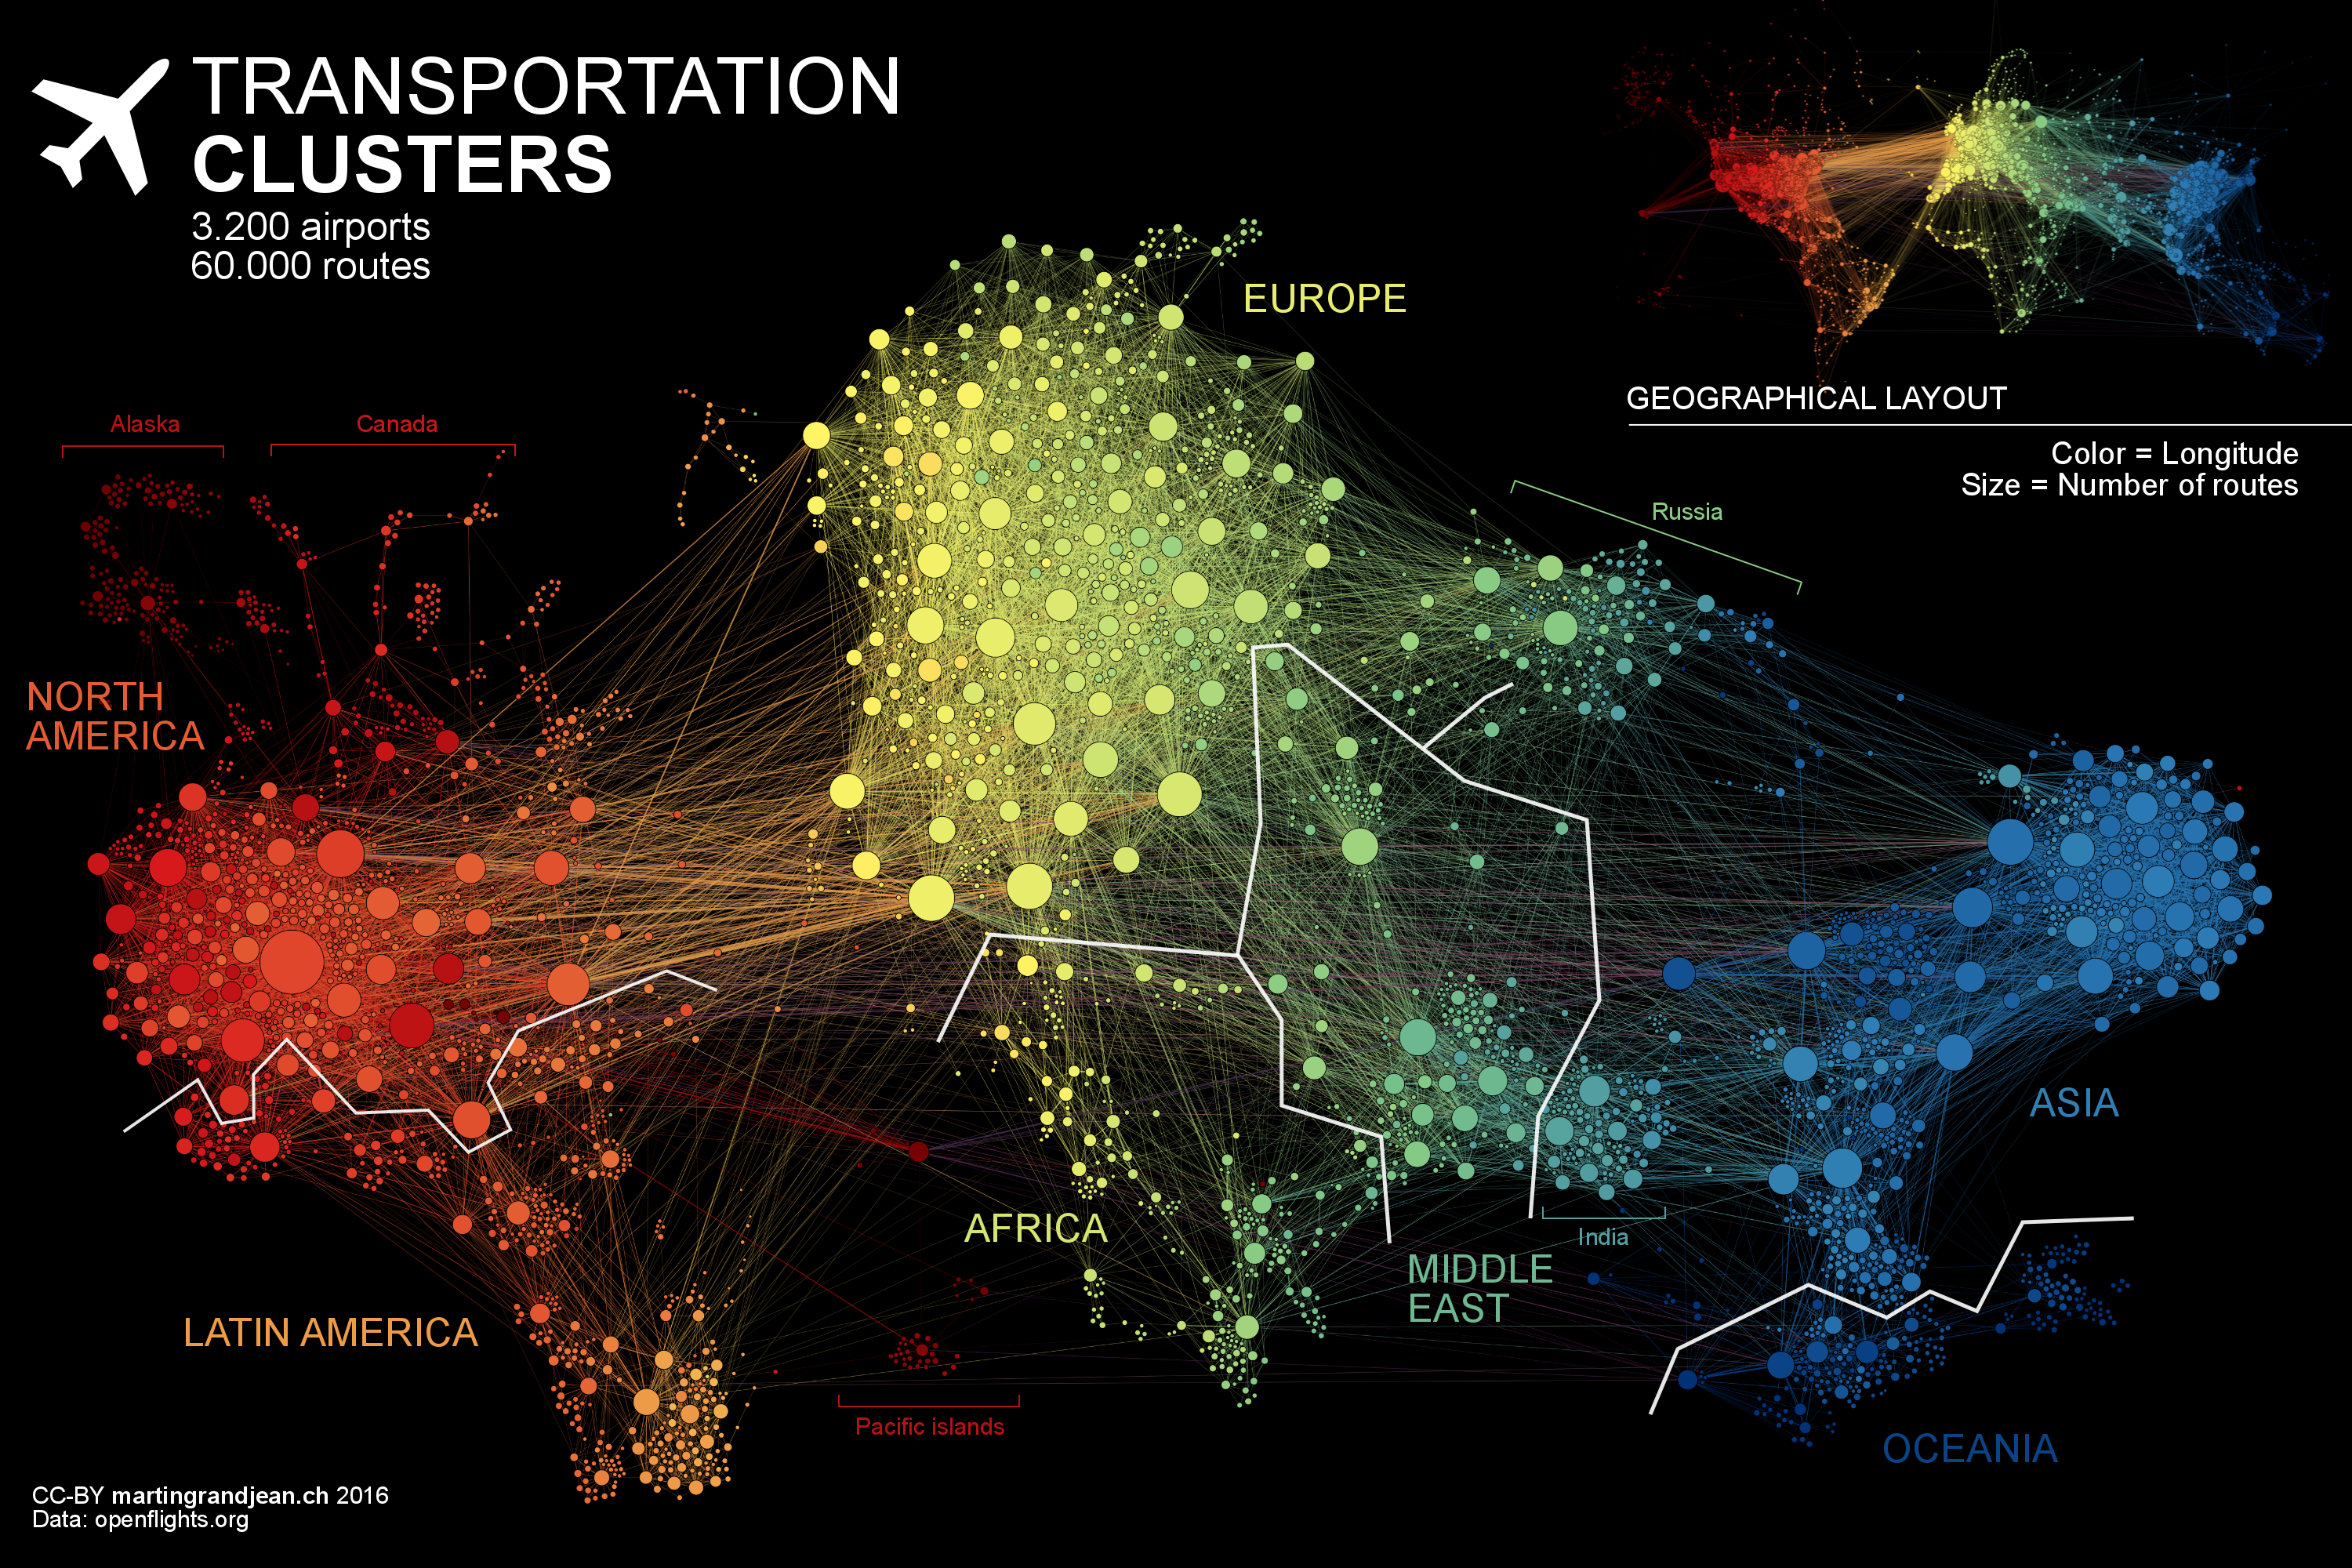
\includegraphics[width=0.95\linewidth, height=0.95\textheight, keepaspectratio]{airports-world-network}\\
\tiny Source: Global transportation map of flight connections (\url{www.martingrandjean.ch})
\end{frame}
%Node size proportional to the number of flight routes

%------------------------------------------------

\begin{frame}
\frametitle{\insertsection}
\centering
\includegraphics[width=\linewidth,height=\textheight,keepaspectratio]{facebook}\\
\tiny Source: Facebook (Mark Zuckerberg, Sept. 2013)
\end{frame}

%------------------------------------------------
\begin{frame}
\frametitle{\insertsection}
\centering
\includegraphics[width=0.9\linewidth,height=\textheight,keepaspectratio]{London Connections Map}\\
\tiny Source: TfL (\url{https://tfl.gov.uk/corporate/transparency/freedom-of-information/foi-request-detail?referenceId=FOI-0525-1920})
\end{frame}

%------------------------------------------------
\begin{frame}
\frametitle{\insertsection}
\centering
\includegraphics[width=0.9\linewidth,height=\textheight,keepaspectratio]{tube}\\
\tiny Source: TfL (\url{https://tfl.gov.uk/modes/tube/})
\end{frame}

%------------------------------------------------

\begin{frame}
\frametitle{\insertsection}
\centering
\includegraphics[width=\linewidth,height=0.8\textheight,keepaspectratio]{disease_net}\\
\tiny Source: The disease-gene network \cite{Goh2007}
\end{frame}

%------------------------------------------------ 
 
\begin{frame}
\frametitle{\insertsection}
\centering
\includegraphics[width=\linewidth,height=0.9\textheight,keepaspectratio]{crime}\\
\tiny Source: Transnational organised crime flow (United Nations Office of Drugs and Crime)
\end{frame}

%------------------------------------------------

\begin{frame}
\frametitle{\insertsection}
\centering
\includegraphics[width=\linewidth,height=0.8\textheight,keepaspectratio]{refugees}\\
\tiny Source: The flight of refugees around the globe (The New York Times, June 20, 2015)
\end{frame}

% Nearly 60 million people are displaced around the world because of conflict and persecution, the largest number ever recorded by the United Nations. About 14 million of those fled in 2014, according to a report released this week.https://www.nytimes.com/interactive/2015/06/21/world/map-flow-desperate-migration-refugee-crisis.html?_r=0

%------------------------------------------------

\begin{frame}
\frametitle{\insertsection}
\centering
\includegraphics[width=\linewidth,height=0.9\textheight,keepaspectratio]{outbreak}\\
\tiny Source: Qualitative outbreak reconstruction (SARS, H1N1) \cite{Brockmann2013}
\end{frame}

%------------------------------------------------

\begin{frame}
\frametitle{\insertsection}
\centering
\includegraphics[width=\linewidth,height=0.9\textheight,keepaspectratio]{covid_network}\\
\tiny Source: COVID-19 epidemic model predictions under different non-pharmaceutical interventions (GPS data) \cite{Firth2020}
\end{frame}

%To ground the simulation in true human interaction patterns, a three-day citizen science experiment was conducted during which the pairwise distances between 469 volunteers in Haslemere (Surry, UK) were tracked continuously using a mobile phone app

%------------------------------------------------

\begin{frame}
\frametitle{\insertsection}
\centering
\includegraphics[width=0.8\linewidth]{bbc_pandemic}\\
\tiny Source: Contagion: The BBC Four Pandemic (2018) - \url{https://youtu.be/RmGiDUczhqQ}
\end{frame}

%------------------------------------------------
\begin{frame} 
\frametitle{\insertsection}
\centering
\includegraphics[width=\linewidth,height=0.8\textheight,keepaspectratio]{mobile}\\
\tiny Source: Spreading patterns of mobile phone viruses \cite{Wang2009}
\end{frame}

%------------------------------------------------

\begin{frame}
\frametitle{\insertsection}
\centering
\includegraphics[width=\linewidth,height=0.8\textheight,keepaspectratio]{disney}\\
\tiny Source: Disney's business strategy in 1957 (`The Disney Recipe', Harvard Business Review, May 28, 2013)
\end{frame}

%------------------------------------------------

\begin{frame}
\frametitle{\insertsection}
\centering
\includegraphics[width=\linewidth,height=0.8\textheight,keepaspectratio]{marvel}\\
\tiny Source: Marvel universe of characters, 'uberframework' (\url{http://www.fastcompany.com})
\end{frame}

%------------------------------------------------

\begin{frame}
\frametitle{\insertsection}
\centering
\includegraphics[width=\linewidth,height=0.9\textheight,keepaspectratio]{food}\\
\tiny Source: Flavour network and the principles of food pairing \cite{Ahn2011}
\end{frame}

%------------------------------------------------
 
\begin{frame}
\frametitle{\insertsection}
\centering
\includegraphics[width=\linewidth,height=0.8\textheight,keepaspectratio]{alliances}\\
\tiny Source: Technology alliances \cite{Schilling2015}
\end{frame}

%------------------------------------------------

\begin{frame}
\frametitle{\insertsection}
\centering
\includegraphics[width=\linewidth,height=0.8\textheight,keepaspectratio]{hidalgo}\\
\tiny Source: Product space \cite{Hausmann2013}
\end{frame}

%------------------------------------------------

\begin{frame}
\frametitle{\insertsection}
\centering
\includegraphics[width=\linewidth,height=0.8\textheight,keepaspectratio]{open_syllabus}\\
\tiny Source: Open Syllabus (\url{https://galaxy.opensyllabus.org})
\end{frame}

%Open Syllabus collects and analyzes one of the largest databases of college course syllabi in the world — as of spring semester 2019, the archive holds 6.9M syllabi from 2,521 colleges and universities in 122 countries, with best coverage in the US, UK, Canada, and Australia. One of the core pieces of metadata extracted from the documents is information about which books and articles are assigned in each course. By analyzing this across millions of classes, we can start to get a bird's-eye view of the relationships among books, articles, and disciplines that emerges from the collective process of teaching and learning encoded by the syllabi.

%------------------------------------------------

\begin{frame}
\frametitle{\insertsection}
\centering
\includegraphics[width=0.9\linewidth,height=\textheight,keepaspectratio]{nature}\\
\tiny Source: Nature (Nov. 2019) -- \url{https://youtu.be/GW4s58u8PZo}
\end{frame}

%------------------------------------------------

\begin{frame}
\frametitle{\insertsection}
\centering
\includegraphics[width=\linewidth,height=0.8\textheight,keepaspectratio]{mapscience}\\
\tiny Source: Map of Science (+20M articles and +2M patents from 1996-2011)\cite{Boyack2014}
\end{frame}

%------------------------------------------------

\begin{frame}
\frametitle{\insertsection}
\centering
\includegraphics[width=\linewidth,height=0.9\textheight,keepaspectratio]{collaboration}\\     
\tiny Source: Co-authorship at the city level (SCOPUS 2008-2012) [\url{http://olihb.com}]
\end{frame}

%------------------------------------------------

\begin{frame}
\frametitle{\insertsection}
\centering
\includegraphics[width=\linewidth,height=0.8\textheight,keepaspectratio]{cruk}\\
\tiny Source: Co-funding in cancer research \cite{Grassano2017}
\end{frame}

%------------------------------------------------

\begin{frame}
\frametitle{\insertsection}
\centering
\Huge ...
\end{frame}

%------------------------------------------------




%=======================================================
%	Why infographics?
%=======================================================
\section{Why infographics?}

%------------------------------------------------

\bgroup
\setbeamercolor{background canvas}{bg = navyblue}
\begin{frame}[plain]{}
\begin{center}
\color{white}{\Huge \insertsection}
\end{center}
\end{frame}
\egroup

%------------------------------------------------

\begin{frame}
\frametitle{\insertsection}

\begin{columns}[c]
\column{.45\textwidth} 
Our ability to {\color{blue}{process images}}
	\begin{itemize}
		\item We have been drawing pictures to {\color{blue}{comunicate}} with each other for thousands of years
		\item Half of our brain is dedicated to {\color{blue}{processing visual signals}}
		\item We can process images {\color{blue}{60,000 times faster}} than text
	\end{itemize}


\column{.45\textwidth}
\centering
\includegraphics[width=5cm]{pont}\\
\tiny{Source: Figurative drawings of the Grotte Chauvet-Pont d’Arc, 30,000-32,000 BP (\url{http://whc.unesco.org/})}
\end{columns}

\end{frame}

%------------------------------------------------

\begin{frame}
\frametitle{\insertsection}

\begin{columns}[c]

\column{.30\textwidth} 
\footnotesize
\centering
\begin{table}
\caption{Students in 2022/23}
\begin{tabular}{lc}
\toprule
\textbf{Student} & \textbf{Course} \\
\hline
Student 1  & SIM    \\
Student 2  & STP    	\\
Student 3  & SD    	\\
Student 4  & SIM    \\
Student 5  & STP    \\
Student 6  & SIM    \\
Student 7  & SD    \\
Student 8  & SIM    	\\
Student 9  & SD    	\\
Student 10 & SD    	\\
Student 11 & SD    \\
Student 12 & SIM \\
\bottomrule
\end{tabular}
\end{table}

\column{.70\textwidth}
\centering
\onslide<2>\includegraphics[width= 0.75\textwidth]{pie}\\
\end{columns}

\end{frame}

%------------------------------------------------

\begin{frame}
\frametitle{\insertsection}
\centering
\includegraphics[width=0.9\linewidth]{money}\\
\tiny{Source: ``Money - A chart of all of it'' (\url{https://xkcd.com/980/})}
\end{frame}

%------------------------------------------------

\begin{frame}
\frametitle{\insertsection}
\centering
\includegraphics[width=0.5\linewidth]{languages}\\
\tiny{Source: ``A world of languages'' (\url{www.scmp.com/infographics/article/1810040/infographic-world-languages})}
\end{frame}

%------------------------------------------------

\begin{frame}
\frametitle{\insertsection}
\centering
\includegraphics[width=0.85\linewidth]{atlas}\\
\tiny{Source: ``Atlas of pollution'' (\url{www.theguardian.com})}
\end{frame}

%------------------------------------------------

\begin{frame}
\frametitle{\insertsection}
\centering
\includegraphics[width=0.54\linewidth]{temperature}\\
\tiny{Source: Monthly global mean temperature compared to average for 1961-1990, Neil Kaye @neilrkaye}
\end{frame}

%------------------------------------------------

\begin{frame}
\frametitle{\insertsection}
\centering
\includegraphics[height = 0.8\textheight]{economist}\\
\tiny{Source: The Economist (September 2019)}
\end{frame}

%------------------------------------------------

\begin{frame}
\frametitle{\insertsection}
\centering
\Large Data, data, data, ... \\
	   \medskip
	   Big Data, Data Science, ...
\end{frame}

%------------------------------------------------

\begin{frame}
\frametitle{\insertsection}

\begin{columns}[c]
\column{.45\textwidth} 

\begin{itemize}
	\item Technological advancements have considerably  increased our capabilities to {\color{blue}{collect}}, {\color{blue}{store}} and {\color{blue}{analyse}} data
	\item Increasing access to data:
	\begin{itemize}
		\item Government data
		\item Open access
		\item Open science
		\item APIs
		\item ...
	\end{itemize}
	\item Risk of information {\color{blue}{overload}}
\end{itemize}

\column{.45\textwidth}
\centering
\includegraphics[width=4.5cm]{byte}\\
\tiny{Source: CNRS (\url{http://www.cnrs.fr/})}

\end{columns}

\end{frame}

%------------------------------------------------

\begin{frame}
\framesubtitle{Data}
\frametitle{\insertsection}
\centering
\includegraphics[width=0.9\linewidth]{moore.png}\\
\tiny{Source: \url{https://ourworldindata.org/technological-progress}}
\end{frame}

%------------------------------------------------

\begin{frame}
\frametitle{\insertsection}
\centering
\includegraphics[width=\linewidth]{bigdata}\\
\tiny{Source: IBM Big Data and Analytics Hub (\url{http://www.ibmbigdatahub.com})}
\end{frame}

%------------------------------------------------

\begin{frame}
\frametitle{\insertsection}
\framesubtitle{Share your examples of infographics}


\begin{enumerate}
	\item Identify an example of infographic
	\item Share your example at\\ \url{https://uofsussex.padlet.org/deggleton/w320creozwtjflkn}
	\item Add your name
	\item Time: 10 minutes
\end{enumerate}

\end{frame}

%------------------------------------------------








%=======================================================
%	Overview of the module
%=======================================================
\section{Overview of the module}

%------------------------------------------------

\bgroup
\setbeamercolor{background canvas}{bg = navyblue}
\begin{frame}[plain]{}
\begin{center}
\color{white}{\Huge \insertsection}
\end{center}
\end{frame}
\egroup

%------------------------------------------------

\begin{frame}
\frametitle{\insertsection}

\begin{columns}[c]

\column{.4\textwidth} 
\centering
\includegraphics[width=4.5cm]{logo}

\column{.6\textwidth}
	\begin{itemize}
	\item 15-credit module
	
	\medskip
	
	\item An option module for all SPRU MSc courses:
		\begin{itemize}
		\item Science and Technology Policy
		\item Strategic Innovation Management
		\item Sustainable Development
		\end{itemize}
		
	\medskip
	
	\item The module introduces students to
		\begin{itemize}
		\item {\color{blue}{qualitative}}, {\color{blue}{quantitative}}, and {\color{blue}{mixed}} methods to collect and analyse network data
		\item principles for generating effective {\color{blue}{infographics}}
		\end{itemize}

	\end{itemize}
	
\end{columns}

\end{frame}

%------------------------------------------------

\begin{frame}
\frametitle{\insertsection}
\framesubtitle{Learning Outcomes}

\centering
\begin{tabular}{lp{5.5cm}l}
\toprule
\multicolumn{2}{l}{\textbf{Learning outcome}} & \textbf{Assessment mode}\\
\hline
\\
1 & 
Explain the concept of network and list the main network indicators & 
ESS\\
\\
2 & 
Describe and apply the major techniques for the collection of network data and their statistical analysis & 
ESS, GPN + GWS\\
\\
3 & 
Identify the main characteristics of networks by means of network measures  & 
ESS, GPN + GWS\\
\\
4 &
Employ network analysis techniques to produce network data-based infographics & 
GPN + GWS\\
\\
\bottomrule
\multicolumn{3}{l}{\scriptsize Note: ESS: Essay; GPN: Group Presentation; GWS: Group Written Submission}\\
\end{tabular}

\end{frame}

%------------------------------------------------


\bgroup
\setbeamercolor{background canvas}{bg = navyblue}
\begin{frame}[plain]{}
\begin{center}
\color{white}{\LARGE This is what you will learn to do ...}
\end{center}
\end{frame}
\egroup

%------------------------------------------------
\bgroup
\setbeamercolor{background canvas}{bg=white}
\begin{frame}[plain]{}
\centering{
\includegraphics[height = 0.95\paperheight, frame]{example1}}
\end{frame}
\egroup

\bgroup
\setbeamercolor{background canvas}{bg=white}
\begin{frame}[plain]{}
\centering{
\includegraphics[height = 0.95\paperheight, frame]{example2}}
\end{frame}
\egroup

\bgroup
\setbeamercolor{background canvas}{bg=white}
\begin{frame}[plain]{}
\centering{
\includegraphics[height = 0.85\paperheight, frame]{example3}}
\end{frame}
\egroup


\bgroup
\setbeamercolor{background canvas}{bg=white}
\begin{frame}[plain]{}
\centering{
\includegraphics[height = 0.85\paperheight, frame]{example4}}
\end{frame}
\egroup

\bgroup
\setbeamercolor{background canvas}{bg=white}
\begin{frame}[plain]{}
\centering{
\includegraphics[height = 0.95\paperheight, frame]{example5}}
\end{frame}
\egroup

\bgroup
\setbeamercolor{background canvas}{bg=white}
\begin{frame}[plain]{}
\centering{
\includegraphics[height = 0.95\paperheight, frame]{example6}}
\end{frame}
\egroup

\bgroup
\setbeamercolor{background canvas}{bg=white}
\begin{frame}[plain]{}
\centering{
\includegraphics[height = 0.95\paperheight, frame]{example7}}
\end{frame}
\egroup

\bgroup
\setbeamercolor{background canvas}{bg=white}
\begin{frame}[plain]{}
\centering{
\includegraphics[height = 0.85\paperheight, frame]{example8}}
\end{frame}
\egroup


%------------------------------------------------

\begin{frame}
\frametitle{\insertsection}
\framesubtitle{Outline}

\centering
\def\arraystretch{1.5}
\begin{tabular}{cl}
\toprule
\textbf{Week} & \textbf{Topic}\\
\hline
1  & Introduction\\
2  & Network definition\\
3  & Network data collection\\
4  & Descriptive network analysis A\\
5  & Descriptive network analysis B\\
6  & Descriptive network analysis C\\
7  & Principles of infographics\\
8  & Network models\\
9  & Innovation networks\\
10 & Social network theories\\
11 & Revisions\\
\bottomrule
\end{tabular}

\end{frame}

%------------------------------------------------

\begin{frame}
\frametitle{\insertsection}
\framesubtitle{Assessment modes}

\textbf{Essay (ESS)} {\color{blue}{[50\% weighting]}}
	\begin{itemize}
	\item 2,500-words essay to present a coherent analysis of the inter-organisational networks 
	\item Data will be provided in Week 5
	\item See Canvas website for more details
	\end{itemize}

\end{frame}

%------------------------------------------------
\begin{frame}
\frametitle{\insertsection}
\framesubtitle{Assessment modes}

\textbf{Coursework}\\
\begin{itemize}
\item Groups up to 3 students
\item Report your group by Week 3: \href{https://docs.google.com/document/d/1y00FtaNSFJkJedAXjxgFTBMlYiI5xIspNkSm8PSipro/edit?usp=sharing}{\smash{https://docs.google.com/document/d/1y00FtaNSFJkJedAXjxgFTBMlYiI5xIspNkSm8PSipro/edit?usp=sharing}}
\item Small-scale network analysis project using novel or existing network data
\item {\color{orange}{Any topic!}}
\item Assessment modes:
	\begin{itemize}
	\item \textbf{Group Written Submission (GWS)} {\color{blue}{[30\% weighting]}}\\
		 Infographic poster (A1-size, PDF)
	\item \textbf{Group Presentation (GPN)} {\color{blue}{[20\% weighting]}}\\
	10-minute video recording presenting the infographic poster (GWS)
	\end{itemize}
\item Submission in Week 11 (see Canvas)
\item Marking criteria (see Canvas)
\end{itemize}

\bigskip

\centering
\includegraphics[width=\linewidth]{flow_chart_group_work}\\

\end{frame}

%------------------------------------------------

\begin{frame}
\frametitle{\insertsection}
\framesubtitle{Assessment modes (RESIT)}

\centering
\def\arraystretch{1.5}
\begin{tabular}{llc}
\toprule
\textbf{Exam} & \textbf{Resit} & \textbf{Weight}\\
\hline
Essay (ESS, 2,500 words)& 
Essay (ESS, 2,500 words)& 
50\%\\

Group Written Submission (GWS) & 
Report (REP, 1,500 words project summary){\color{orange}{*}} &
30\%\\
Group Presentation (GPN) &
Project (PRJ, A1-size poster){\color{orange}{*}}&
20\%\\

\bottomrule
{\color{orange}{*Individual work}}
\end{tabular}


\end{frame}

%------------------------------------------------

\begin{frame}
\frametitle{\insertsection}
\framesubtitle{Readings}

\begin{itemize}
	\item Essential and recommended readings as listed Canvas
	\item {\color{blue}{Selected chapters}} from the below books
\end{itemize}
\medskip
\medskip

\centering
\includegraphics[height=4.5cm, frame]{wassermancover}\hspace{0.5cm}
\includegraphics[height=4.5cm, frame]{igraphcover}\hspace{0.5cm}
\includegraphics[height=4.5cm, frame]{tufte}
\end{frame}

%------------------------------------------------

\begin{frame}
\frametitle{\insertsection}
\framesubtitle{Software packages}


\begin{itemize}
	\item {\color{blue}{R}} (\url{www.r-project.org}) and {\color{blue}{R-Studio}} (\url{www.rstudio.com})
	\item {\color{blue}{igraph}} package for R (\url{http://igraph.org/r/})
	\item {\color{blue}{Gephi}} (\url{https://gephi.org/})
	\item {\color{blue}{VOSviewer}} (\url{www.vosviewer.com})
\end{itemize}
\medskip
\medskip

\centering
\includegraphics[height=1cm]{../_shared_pics/r_logo} \hspace{1cm}
\includegraphics[height=1cm]{../_shared_pics/rstudio_logo} \hspace{1cm}
\includegraphics[height=1cm]{../_shared_pics/igraph_logo}
\medskip

\includegraphics[height=1cm]{../_shared_pics/gephi_logo} \hspace{1cm}
\includegraphics[height=1cm]{../_shared_pics/vos_logo} 
\end{frame}

%------------------------------------------------

\begin{frame}
\frametitle{\insertsection}
\framesubtitle{Canvas website}
\centering
\includegraphics[width=0.8\linewidth, frame]{canvas}
\end{frame}

%------------------------------------------------







%=======================================================
%	Next time ...
%=======================================================
\section*{Next time ...}
%------------------------------------------------

\begin{frame}
\frametitle{\insertsection}

\begin{itemize}
\item 	\textbf{Seminar: Introduction}
		\begin{itemize}
		\item Network visualisation exercise
		\item Familiarising with the concept of network
		\end{itemize}
\medskip
\medskip
\item 	\textbf{Lecture: Network definition}
		\begin{itemize}
		\item Definition of network and different types of networks
		\item Overview of the historical and disciplinary origins of (social) network analysis
		\item Network visualisation standards
		\item Overview of R and the igraph package 
		\end{itemize}
\end{itemize}



\end{frame}

%------------------------------------------------



%=======================================================
%	Questions
%=======================================================
\bgroup
\setbeamercolor{background canvas}{bg = orange}
\begin{frame}[plain]{}
\begin{center}
\color{white}{\Huge Questions}
\end{center}
\end{frame}
\egroup



%=======================================================
%	References
%=======================================================
\begin{frame}[allowframebreaks]
\frametitle{References}

\tiny
\bibliographystyle{apalike}
\bibliography{library.bib}
%\bibliography{references.bib}
\end{frame}
%=======================================================


\end{document}